\section{Kommunikationskostenoptimierung}
\hyphenation{High--Per-for-mance}
\hyphenation{Per-for-mance}
\hyphenation{Com-pu-ting}
\hyphenation{Be-rech-nungs-eng-pass}
Es sollen Strategien zur Reduktion von Kommunikationskosten bei der Umsetzung der 3D-FFT in einer High-Performance Architektur behandelt werden.\\

Die Kommunikation findet im High-Performance Kontext zwischen verschiedenen Prozessen/Prozessoren statt, deren lokale Daten aktualisiert werden müssen.\\
Kommunikationskosten sind dabei die verwendeten Aufwände in Zeit für Synchronisationsabschnitte zwischen einzelnen Datenverarbeitungsschritten.\\

\begin{figure}
\centering
  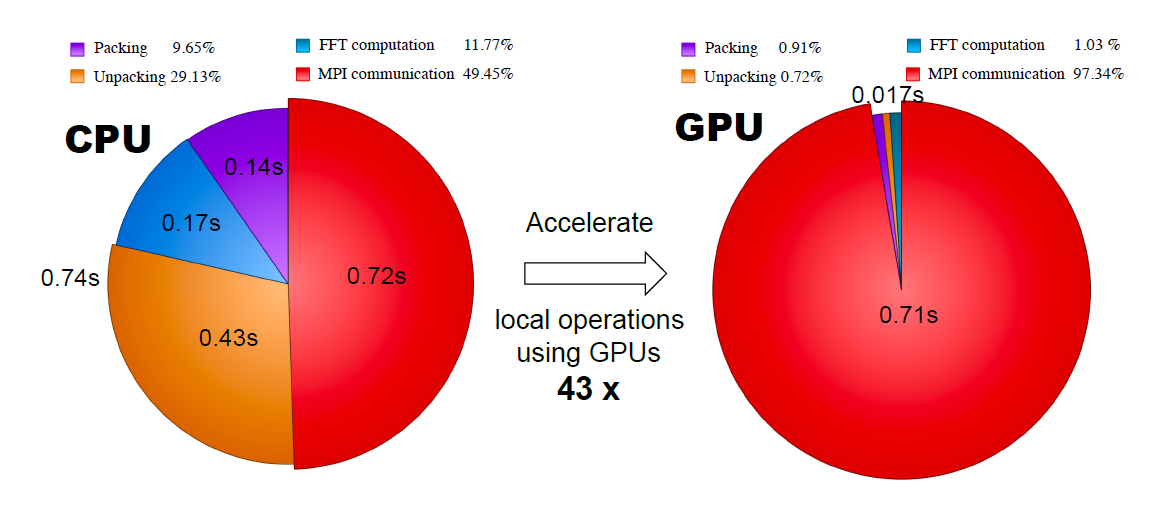
\includegraphics[width=\linewidth]{res/speedup.png}
  \caption{\cite[Abb. 3]{mainpaper} Kreisdiagramme zur Visualisierung von Erfolgen und Bottlenecks bei der GPU Beschleunigung von 3D-FFTs}
  \label{fig:speedup}
\end{figure}

Dieser Schritt wird durch entstehende Kommunikationsengpässe motiviert, welche nach der alleinigen Prozessorbeschleunigung auftreten können.\\
Exemplarisch zeigt die Quelle \cite[Abb. 3]{mainpaper} einen solchen Kommunikationsengpass (siehe Abbildung \ref{fig:speedup}).
Die durch die Verwendung von GPUs statt CPUs erreichte Beschleunigung durch Parallelismus optimiert dort alle Programmanteile um ein vielfaches mit der Ausnahme der Kommunikation.\\

Wie Abbildung \ref{fig:speedup} zeigt hat sich bei dem in der Quelle durchgeführten Experiment die Zeit, welche im FFT-Algorithmus für Kommunikation zwischen den GPU's/CPUs aufgewendet wird, nur vernachlässigbar verändert. Alle anderen Aktionen (Unpacking, Processing, Packing) haben sich erheblich durch Parallelisierung mit GPUs beschleunigt ($ \frac{0.74s}{0.017s} \approx 43.5$-fache Beschleunigung).\\
\\
Wird Kommunikationszeit mitbetrachtet ist die Beschleunigung $\frac{0.14s+0.17s+0.42s+0.72s}{0.017s+0.71s}=200,8\%$, also nur 2-fach.

Prinzipiell ist Kommunikation ebenfalls parallelisierbar. Da Kommunikation jedoch der Verbreitung einer frisch errechneten, neuen Wahrheit auf anderen Prozessoren dient, hängt der Grad der Parallelisierbarkeit direkt an der unmittelbaren Wichtigkeit dieser Wahrheit für weitere Berechnungsschritte.\\
Diese Eigenschaft macht Kommunikation hinsichtlich der beteiligten Prozesse oft zu einem inherent seriellen, d.h.~in einem gewissen Grad nicht parallelisierbaren Problemanteil.\\
Inherente serielle Anteile in einer Problemstellung limitieren den möglichen maximalen Speedup durch Parallelisierung der gesamten Applikation.\\
Diese Sachverhalte können am FFT-Problem bei der Einteilung in Phasen beobachtet werden: In einer Phase werden auf $N$ Prozessen insgesamt $N$ \textit{Pencil}s berechnet. Die Input-\textit{Pencil}s für die folgende Phase setzten sich aus den Teilergebnissen aller Vorgängerschritte zusammen. Es müssen demnach für die nächste Phase alle Ergebnisse der vorigen Phase bereits verfügbar sein, voraus Serialität folgt.\\
Da Kommunikation unter dem vorgesetzten Ziel der Multi-Prozessorbeschleunigung der Applikation FFT unvermeidbar ist und die Kommunikation selbst zum Berechnungsengpass führt, muss weiter die Optimierung der Kommunikation behandelt werden.\\
\\
In diesem Papier wird die Quelle \cite{mainpaper} für Beispiele von Experimenten und Lösungsansätzen herangezogen. Zum weiteren Verständnis sollen demnach zunächst die in der Quelle verwendeten Technologien, Systemarchitekturen und Spezialbegriffe erläutert werden.\\
Daraufhin behandelt dieses Werk konzeptionelle Lösungsansätze und erläutert und relativiert diese mit den Experimenten aus der Quelle.


\subsection{Summit Supercomputer}
Der Summit-Supercomputer dient für alle im Folgenden beschriebenen Experimente als Durchführungsplattform. Für Betrachtungen hinsichtlich Kommunikationsfähigkeit sind daher Kenntnisse über den Summit Supercomputer von Nutzen.\\

Der Summit-Supercomputer im Oak Ridge National Laboratory, Tennessee, USA, ist ein Multi-Prozessor-Supercomputer, der seit 2018 in Betrieb ist. Der Verwendungszweck des Rechners ist der Einsatz in der Wissenschaft.

\subsubsection{Komponenten}

\begin{figure}
\centering
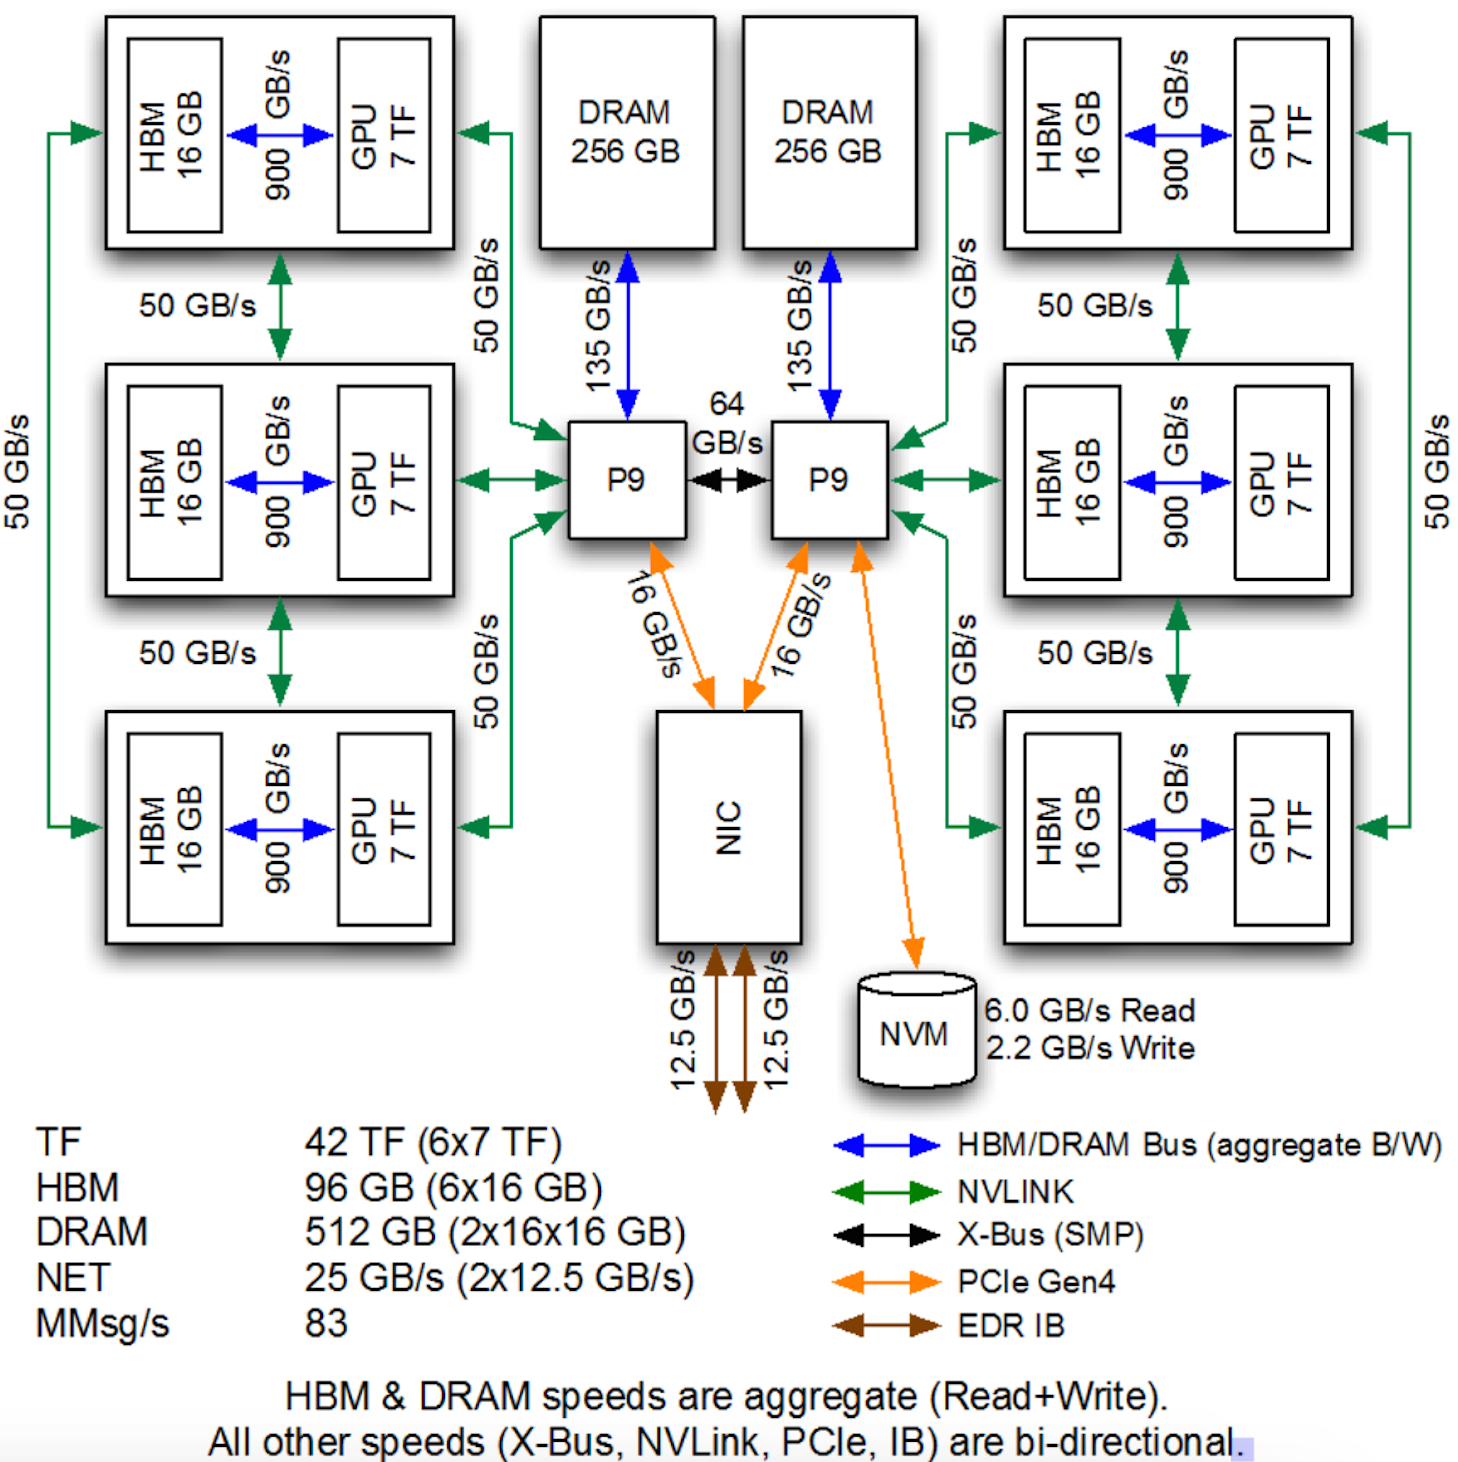
\includegraphics[width=0.6\textwidth]{res/architecture.png}
\caption{\cite[Abb. 1]{mainpaper} Aufbau eines Knotens des Summit Supercomputers, verwendete Kommunikationstechnologien und Komponenten}
	\label{fig:architecture}
\end{figure}
\begin{enumerate}
	\item 4608 Knoten gesamt
	\item je 2 CPUs (IBM POWER9, in der Graphik unter P9)
	\item je 6 GPUs (NVIDIA Volta V100s)
\end{enumerate} \cite{osummit}
Abbildung \ref{fig:architecture} zeigt die generelle Systemarchitektur eines Knotens des Summit-Rechners.\\
Eine CPU und 3 GPU's sind auf einem Knoten unter einem CPU-Sockel zusammengefasst. Es befinden sich 2 solcher Sockel auf einem Summit-Knoten. Zwischen allen Prozessoren unter einem Sockel existieren P2P Verbindungen mit der NVLink Verbindungstechnologie.\\
Die Komponenten sollen weiter als Einheiten von Rechenressourcen angesehen werden. Diese Einheiten sind:
\begin{enumerate}
	\item Knoten
	\item Sockel
	\item Prozessor
\end{enumerate}

Terminologie zur Unterscheidung von Kommunikationsvorgängen zwischen und innerhalb Sockeln wird wie folgt definiert:\\
\begin{defi}[Knoteninterne Kommunikation (eng. \textit{same-socket-communication})].
Kommunikationsvorgänge, welche zwischen Prozessoren unter dem selben Sockel erfolgen.
\end{defi}
\begin{defi}[Knotenübergreifende Kommunikation (eng. \textit{cross-socket-communication})]
Kommunikationsvorgänge, welche zwischen Prozessoren auf unterschiedlichen Sockeln erfolgen.
\end{defi}
Für sockelübergreifende Kommunikation auf einem Knoten existiert ein X-Bus (64GB/s), der zwischen den CPUs angelegt ist.\\
Theoretisch können also maximal $\frac{64GB/s}{50GB/s} = 1.28$ Prozessoren sockelübergreifend socket kommunizieren.\\
Unter der Annahme, dass jeder Prozessor im Schnitt mit jedem anderen Prozess gleich viel kommuniziert  entstehen demnach Kommunikationsengpässe zuerst bei der sockelübergreifenden Kommunikation.\\
In den in diesem Papier beschriebenen Experimenten treten potentiell beide dieser Arten der Kommunikation auf.

\subsubsection{Topologie}
Die Knoten sind untereinander unter einer bestimmten Topologie verbunden. Am Summit-Rechner wurde die Fat-Tree Topologie verwendet.\\
\begin{figure}
\centering
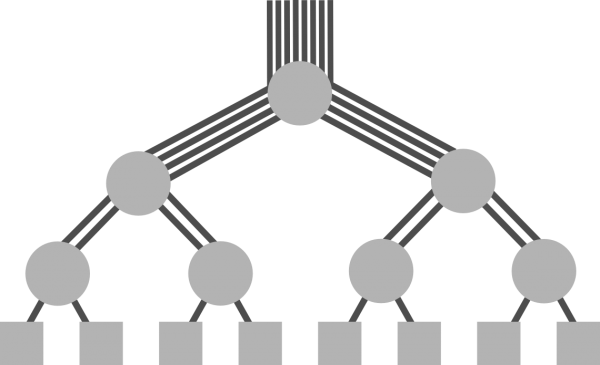
\includegraphics[width=0.4\textwidth]{res/fat_tree.png}
\caption{\cite{fattree} Graphische Darstellung der Fat-Tree Topologie}
	\label{fig:fat_tree}
\end{figure}
Ein Fat-Tree ist eine Topologie, bei der Switches zu einem Binärbaum verknüpft werden. Endknoten, also Summit-Knoten, werden dabei an den Blättern des Baumes platziert.\\
Maßgeblich für den Fat-Tree ist dabei die Regel, dass für jeden Switch im System die Anzahl der Verbindungen nach unten gleich der Anzahl der Verbindungen nach oben ist, also für jeden Knoten gleich viel Bandbreite zu den Eltern wie zu der Gruppe aller Kinder verfügbar ist. Daraus folgt die Anzahl der Verbindungen pro Switch in Abhängigkeit der Baumhöhe $h$, maximaler Baumhöhe $h_{max}$, Der Höhe am Wurzelknoten $h_{root}=0$ und der Anzahl der Elternverbindung eines Blattknotens $c$ (hier: $c=1$):
\begin{itemize}
	\item Anzahl Elter-/Kindverbindungen : $(h_{max}+1-h)*c$
	\item Anzahl Verbindungen pro Kind : $\frac{(h_{max}+1-h)*c}{2}$ bei 2 Kindern
\end{itemize}
Die Anzahl an Verbindungen ist daher maximal am Wurzelknoten mit $h_{max}+1$, der Baum wird zur Wurzel hin \glqq dicker (eng. \textit{fat})\grqq.\\
Hält eine Fat-Tree Topologie das Verhältnis von Eltern- zu Kindverbindung von $1:1$ ein, nennt man diese Non-Blocking. Die Gegenteilige Blocking-Eigenschaft ist bei Nichteinhaltung festzustellen.\\
Ist das Verhältnis unausgeglichen ist die Kommunikation durch den konkreten unausgeglichenen Switch limitiert. Zum Beispiel könnten doppelt so viele Kindverbindungen existieren als Elternverbindungen ($1:2)$. So können verhältnismäßig viele Kindknoten über den Switch zeitgleich kommunizieren, jedoch kann nur die Hälfte aller Kindkommunikation an Eltern weitergereicht werden. Man spricht bei diesem Beispiel von einem Blocking-Faktor von 2, Kind zu Eltern.\\
\\
Die Topologie erreicht durch das exponentielle Wachstum von Blattknoten des Binärbaumes mit der Baumtiefe leicht eine große Anzahl verknüpfbarer Prozessoren ($2^h_{max}$). (vgl. \cite{fattree})\\
\\
Man vergleiche mit Abbildung \ref{fig:fat_tree}.

\subsection{Relevante Technologien}
Es werden weiter relevante Technologien benannt und beschrieben. Die Relevanz ergibt sich teils durch die Präsenz der Technologie am Summit-Rechner und die dadurch bstehende Verwendung in den in der Quelle \cite{mainpaper} beschriebenen Experimenten.

\subsubsection{ NVLink }
Eine proprietäre Verbindungstechnologie auf Prozessorebene, entwickelt von NVIDIA.\\
Traditionell kommunizierten Prozessoren in einer Systemarchitektur ausschließlich über den PCIe-Bus. NVLink erlaubt zusätzliche P2P Verbindungen zwischen Prozessoren und verbessert durch diese Direktkommunikation die kommunikativen Eigenschaften der gesamten Systemarchitektur (vgl. \cite{nvlink}).\\
\\
Unidirektional bietet die Technologie bei den verwendete Prozessoren 25GB/s. Die Technologie ist allerdings konzeptionell bidirektional, wodurch die in Abbildung \ref{fig:architecture}, d.h. \cite[Abb. 1]{mainpaper}, 50GB/s zu Stande kommen.\\
Auf der Website des Summit-Rechners wird allerdings angegeben, dass zwischen 2 Prozessoren auf einem Sockel im Summit Supercomputer 2 NVLink-Verbindungen angelegt sind, was die Bandbreite theoretisch auf 100GB/s anhebt (vgl. \cite[FAQ, What is NVLink?]{osummit}).\\
Es besteht daher eine Diskrepanz zwischen den Quellen.

\subsubsection{ NVIDIA GPUDirect }
NVIDIA GPUDirect-Storage ist Term für Speichersysteme auf NVIDIA Grafikkarten, die den direkten Speicherzugriff bei Grafikkarten ohne den traditionellen Umweg über den CPU-RAM ermöglichen. Dieser Vorgang wird als \textit{Remote Direct Memory Access (RDMA)} bezeichnet.\\
Es können dabei verschiedene Arten von Päripherie verbunden werden, welche dann direkt GPU-Speicher lesen und schreiben können. Somit können die Päriperien direkt mit den GPUs kommunizieren.\\
Beispiele für Päripherien sind Netzwerkadapter, Speicher (wie Solid State Drives) und andere Graphikkarten (vgl. \cite{gpud}).\\
Die GPUDirect Technologie wir am Summit zur Beschleunigung von MPI-Kommunikation zwischen Grafikkarten eingesetzt (vgl. \cite[Kap. 1]{mainpaper}).

\subsubsection{ \textit{Message Passing Interface} (MPI) }
MPI ist ein Standard, der Schnittstellen für den Nachrichtenaustausch zwischen Prozessen spezifiziert.\\
Portabilität und Einfachheit werden als primäre Ziele angegeben (vgl. \cite[Kap. 1.1]{mpi}).\\
Es gibt mehrere Implementierungen dieses Standards, zum Beispiel die Open-Source-Variante OpenMPI (\cite{openmpi}).\\
In verteilten Systemen, wie z.B.~ dem Summit-Rechner, wird MPI als Abstraktion für die Kommunikation zwischen parallelen Prozessoren/Prozessen verwendet.\\
MPI wird in den in diesem Papier beschriebenen Experimenten als Kommunikationsschnittstelle verwendet.

\subsubsection{ CUDA }
Die \textit{\textbf{C}ompute \textbf{U}nified \textbf{D}evice \textbf{A}rchitecture (CUDA)}, entwickelt von NVIDIA ist eine Plattform und Programmiermodell für parallele Berechnungen auf NVIDIA GPUs (vgl. \cite{cuda}).\\
Die Technologie gewährt niedrigabstrakten Zugriff auf Rechenressourcen von NVIDIA Grafikprozessoren und ermöglicht so performante Implementierungen.\\
Da der Summit-Rechner NVIDIA-GPUs verwendet wird CUDA in den in diesem Papier beschriebenen Experimenten teilweise für Interprozessorkommunikation eingesetzt.\\
Der Einsatz der Technologie wird bei den im Folgenden gezeigten Experimenten evaluiert.


\subsubsection{ CUDA-aware MPI }
Ist eine Kombination aus CUDA und MPI.\\
Da CUDA mit dem MPI Standard kompatibel ist, sind MPI-Implementierungen durch CUDA möglich.\\
CUDA-aware MPI verwendet diese alternativen Imlementierungen und ermöglicht die Verwendung von CUDA-Konstrukten, wie z.B. GPU-Buffer, nativ in MPI-Aufrufen alternativ zum herkömmlichen Host/CPU-Buffer. Auf diese Weise wird wieder der Umweg über den CPU-RAM vermieden (\cite{cudampi}).\\
Die resultierende MPI-Implementierung ist niedrigabstakt und plattformspezifischer und stellt dadurch in vielen Fällen eine bessere, performantere Umsetzung des MPI-Standards im Speziellen für NVIDIA GPUs dar.\\
Im Kontext dieses Papiers ist CUDA-aware MPI eine Option als verwendbare Kommunikationstechnologie.

\subsection{Weitere spezielle Terminologie}
Im Kontext der hier beschriebenen Experimente und verwendeter Technologien werden einige spezielle Begriffe verwendet, die im Folgenden genauer erläutert werden sollen.

\subsubsection{MPI\_All2All}
\textit{MPI\_Alltoall} (Auch: A2A, All2All, AllToAll) ist eine Kommunikationsroutine des Message Passing Interface Standards. Dabei Senden alle $N$ beteiligten Prozesse Nachrichten der selben Größe zu allen $N$ Prozessen (inklusive dem eigenen Prozess). Der Kommunikationsaufwand beträgt also $N^2 * Nachrichtenl"ange$.\\
Es wird in jedem Prozess ein Kommunikationspuffer verwendet, dessen Größe $N*Nachrichtenl"ange$ beträgt. (vgl. \cite{MPImanpage})\\

\subsubsection{MPI P2P}
Als Peer to Peer (P2P) Kommunikation bezeichnet man eine Kommunikationsstrategie, bei der alle nötigen Informationen von einem kommunizierenden Knoten zum anderen direkt und nach Bedarf ausgetauscht werden. 
Dabei sind die Parameter der konkreten Kommunikation prinzipiell an keine weiteren Eigenschaften gebunden.\\
Die Quelle, aus der die hier behandelten Experimente stammen (\cite{mainpaper}) und die MPI P2P als Kommunikationsroutine benennt, geht nicht auf die genaue Realisierung dieser ein. Da der MPI-Standard keine dedizierte P2P-Funktion zu definiert, wird an dieser Stelle angenommen, dass diese Art der Kommunikation durch MPI\_Send und MPI\_Recv aufrufen realisiert wird, welche als die nativen, d.h.~niedrigabstraktesten Sende-/Empfangbefehle in MPI zu verstehen sind.\\
Es handelt sich im Kontext von MPI bei P2P hier also um Einzelnachrichten ohne eine besondere Kommunikationsstrategie.\\

\subsubsection{Kommunikationsrichtung}
\begin{defi}[Unidirektionale Kommunikation (\textit{ eng. unidirectional communication })]
In einem abgeschlossenen Kommunikationsvorgang zwischen den Prozessen $p1$ und $p2$ werden Daten ausschließslich von $p1$ nach $p2$ kommuniziert.
\end{defi}
\begin{defi}[Bidirektionale Kommunikation (\textit{ eng. bidirectional communication })]
In einem abgeschlossenen Kommunikationsvorgang zwischen den Prozessen $p1$ und $p2$ können Daten sowohl von $p1$ nach $p2$, als auch von $p2$ nach $p1$ gleichzeitig ausgetauscht werden.
\end{defi}

\subsubsection{3D-FFT Datenkomposition}
Der Input der 3D-FFT ist ein 3D-Tensor. Es ist abhängig von Algorithmus, welche Teile der Inputdaten für welchen Verarbeitungsschritt benötigt werden.
Durch eine effiziente Bündelung von Operation und Daten für die verschiedenen Schritte des Algorithmus können Kommunikationskosten eingespart werden.\\
Im Kontext des Datentensors der 3D-FFT wird von folgenden Datenkompositionen gesprochen:
\begin{enumerate}
	\item \textit{pencil}\\
		Zu Deutsch Stift, suggeriert einen eindimensional ausgedehnten Anteil am Tensor, also ein 3D Tensor mit einer der Dimensionen $\{1,1,N\},\{1,N,1\},\{N,1,1\}$.
	\item \textit{slab}\\
		Zu Deutsch Platte, suggeriert einen zweidimensional ausgedehnten Anteil am Tensor, also ein 3D Tensor mit einer der Dimensionen $\{N,N,1\},\{N,1,N\},\{1,N,N\}$.
\end{enumerate}

\subsection{Lösungsansätze}
Konzeptionell gibt es 2 Optionen um Kommunikationskosten zu verringern.
\begin{itemize}
	\item Option 1: Verwendung eines besseren Algorithmus hinsichtlich serieller Anteile und Kommunikation.
	\item Option 2: Verbesserung der Kommunikationsstrategie unter Einbeziehung von Eigenschaften der Systemarchitektur.
\end{itemize}
Es sollen im Folgenden konkrete Lösungsansätze genannt und an Beispielen aus der Quelle \cite{mainpaper} gezeigt werden.

\subsubsection{Ermittlung tatsächlicher Bandbreiten}
Im Sinne von Option 2 werden Kommunikationsbenchmarks auf dem Ausführungsrechensystem durchgeführt. Dieser Schritt dient der Informationsgewinnung über die Kommunikativen Eigenschaften des Ausführungssystems. Es werden dadurch die tatsächlich verfügbaren Bandbreiten bei verschiedenen Umständen in der Komunikation ermittelt.\\
Sollten bei der initialen Recherche über das System Systemeigenschaften übersehen worden sein oder sind nichttriviale Effekte hinsichtlich Kommunikation vorhanden, kann durch die Informationsgewinnung in diesem Schritt entsprechend reagiert werden.
Eine Art der Ermittlung der Bandbreiten ist die Erzeugung gleichverteilter, randomisierter Kommunikationslast unter verschiedenen Bedingungen und anschließender Messung der Performanz.\\
\begin{figure}
\centering
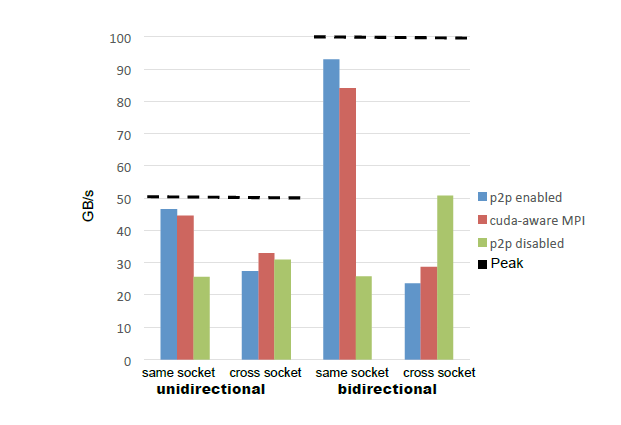
\includegraphics[width=0.6\textwidth]{res/bench0.png}
\caption{\cite[Abb. 4]{mainpaper} Benchmark der Bandbreite für verschiedene Möglichkeiten der P2P Kommunikation}
	\label{fig:bench0}
\end{figure}
Untersuchungen sind
\begin{itemize}
	\item same-socket vs. cross-socket
	\item unidirectional vs. bidirectional
	\item p2p vs. CUDA-aware MPI vs. p2p deaktiviert
\end{itemize}
Dieses Verfahren wurden im Papier \cite{mainpaper} durchgeführt. Das Ergebnis ist in \ref{fig:bench0} zu betrachten.\\
Es wurde dort am meisten Durchsatz sockelintern (same-socket), bidirectional über non-cuda p2p erreicht, dicht gefolgt von der cuda-aware Variante.\\
Das Ergebnis macht theoretisch Sinn: Die zwischen den Prozessoren verwendete sockelinterne NVLink Verbindungstechnologie am Summit-Rechner erlaubt verlustfrei bidirektionale Datenübertragung. Der daraus folgende theoretische Effekt von insgesamt doppelter Bandbreite ist in Abbildung \ref{fig:bench0} am Unterschied zwischen bidirektionaler und unidirektionaler Kommunikation erkennbar.\\

\subsubsection{Auswahl einer Kommunikationsstrategie}
\begin{figure*}
	\begin{subfigure}[t]{0.5\textwidth}
		\centering
		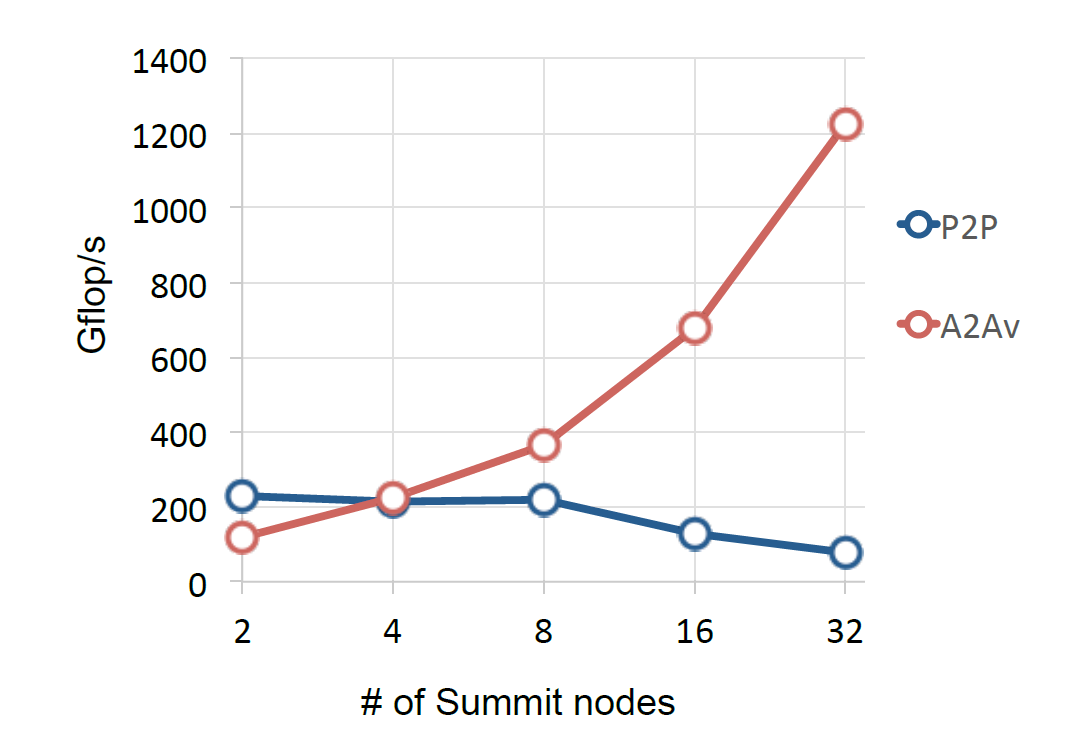
\includegraphics[width=1\textwidth]{res/bench.png}
		\caption{\cite[Abb. 5]{mainpaper} Benchmark P2P vs A2A Gflops/s \& Anzahl Knoten}
		\label{fig:bench}
	\end{subfigure}
~
	\begin{subfigure}[t]{0.5\textwidth}
		\centering
		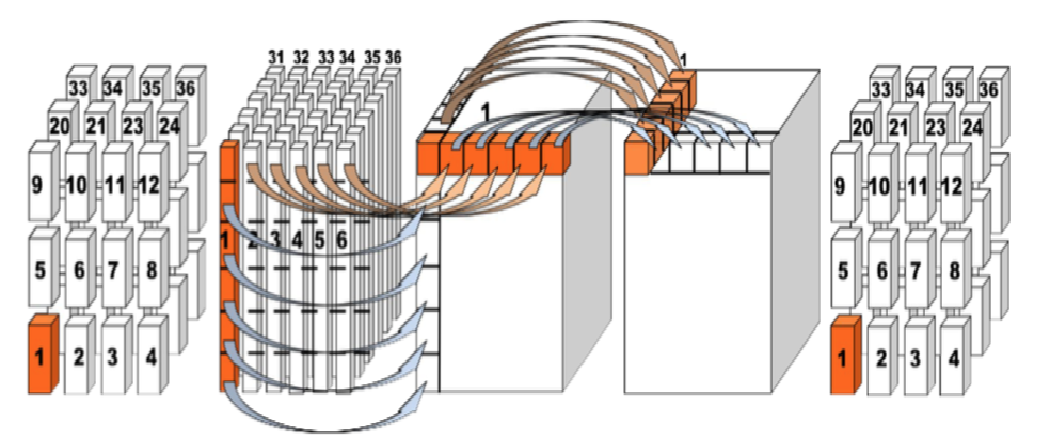
\includegraphics[width=1\textwidth]{res/algo.png}
		\caption{\cite[Abb. 2]{mainpaper} Prinzipieller Aufbau des 3D-FFT Algorithmus. }
		\label{fig:algo}
	\end{subfigure}
	\caption{Zwei begleitende Abbildungen zu Lösungsansätzen 1 und 2}
\end{figure*}

In MPI stehen viele Kommunikationsstrategien zur Verfügung. Verschiedene Kommunikationsstrategien zeigen problem- und systemabhängig unterschiedliche Performanzen. Zu sehen ist dies Beispielhaft in \ref{fig:bench}.
Es lohnt sich daher, geeignete Strategien zu finden. Das kann durch theoretische Überlegung geschehen, praktisch sind allerdings oft nichttriviale Effekte zu verzeichnen. Da praktische Ermittlung durch Benchmarking ist daher ein bewährter Ansatz.\\
Dieser Ansatz ist konzeptionell Option 2 zuzuordnen.\\
\\
Abbildung \ref{fig:bench}, welche sich auf einen solchen Benchmarking-Versuch aus der Quelle \cite{mainpaper} bezieht, zeigt das Verhältnis zwischen den erreichten Gflops/s zu der Anzahl der Verwendeten Knoten am Summit.\\
Verwendete Strategien sind:
\begin{enumerate}
	\item MPI Alltoall
	\item MPI P2P
\end{enumerate}
P2P ist schneller bei der Verwendung 4 Knoten oder weniger, die generelle Effizienz (Anzahl Gflops/s) sinkt jedoch mit der Anzahl an Knoten ab.\\
All2All skaliert generell jedoch besser und zeigt bei mehr als 4 Knoten deutlich bessere Ergebnisse. Die generelle Effizienz (Anzahl Gflops/s) steigt sogar mit der Anzahl der Knoten.\\
Die Quelle, in der die Ergebnisse des Experiments beschrieben sind (\cite{mainpaper}), geht jedoch selbst weiter nicht auf eine mögliche Begründung ein.\\
Eine triviale, wenn auch spekulative Begründung ist der Einsatz von Scheduling. In einem Multi-Prozessor-System wie dem Summit-Rechner wird üblicherweise Kommunikation einem Scheduling unterzogen. Bei der Verwendung von P2P werden viele einzelne Nachrichten erzeugt, welche keine weiteren Regeln, Strategien oder Intentionen an den Scheduler mitteilen. Das Scheduling verläuft daher nach dem \glqq besten Bemühen\grqq(\textit{best effort}) prinzip. P2P Kommunikation sollte demnach mehr Last im Scheduler erzeugen als A2A, da A2A eine geregelte Strategie innehat, die dynamische Scheduling-Lasten vermindert. Das kann die Gesamtapplikation verlangsamen.\\
\\
Bei diesem Lösungsansatz wurde die Superiorität von All2All in Punkten Zeit und Skalierbarkeit für das 3D-FFT-Problem festgestellt.\\
Dieses Ergebnis ist theoretisch Sinnvoll, da, wie die Abbildung \ref{fig:algo} zeigt, All2All Kommunikation die Bedürfnisse der 3D-FFT Applikation nahezu exakt abbildet.\\
Sei ein \textit{Pencil} der Länge $N$ gegeben, so erzeugt ein Prozess $N$ Werte für $N$ Folgeprozesse. Auf den Folgeprozessen wird aus den Teilergebnissen (einzelne Werte) ein neuer \textit{Pencil} der Länge $N$ zusammengefügt.\\
In All2All Kommunikation wird ein Buffer der Länge $N$ angelegt. Dieser Buffer wird durch die 1D-FFT Operation befüllt. Die einzelnen Werte werden durch All2All an die Folgeprozesse verteilt.

\subsubsection{Algorithmische Änderung}
Im Sinne von Option 1 kann der verwendete Algorithmus durch einen mit besseren kommunikativen Eigenschaften ausgetauscht werden.\\
Bei einem hohen Kommunikationsanteil, wie der in dem hier angesprochenen Beispiel von $>97\%$, lohnt sich dabei sogar eine Erhöhung der Rechenzeit für das reine FFT-Problem als Trade-off für verringerte Kommunikationslast.\\
\\

Dieser Ansatz wird auch in der Quelle \cite{mainpaper} verfolgt:
Der zuerst vorgestellte Algorithmus agiert in folgenden Phasen:
\begin{itemize}
	\item[1] Transformiere X-Richtung des Tensors
	\item[2] Transformiere Y-Richtung des Tensors
	\item[3] Transformiere Z-Richtung des Tensors
	\item[4] Rückbewegung in die ursprüngliche Ausrichtung
\end{itemize}
(vgl. Abbildung \ref{fig:algo})\\
Zwischen den Phasen wird kommuniziert. Die Kommunikation verhält sich zu den jeweiligen Phasen sequenziell, d.h.~ist nicht mit einer Phase parallelisierbar, oder fähig zu Pipelining.\\
Können die kommunikativen Anteile der Phasen zusammengefasst werden ergibt sich daraus weniger redundante, serielle Kommunikation.\\
Hier wird dies in Form von \textit{Slab}-Datenkomposition durchgeführt.
Zuvor erhielten Prozesse eine Dimension des 3D-FFT-Input Datentensors nach der \textit{Pencil}-Datenkomposition, auf dem eine 1D-FFT berechnet wird. Dann werden die Ergebnisse propagiert und dabei der Tensor Transformiert.\\
Für diesen Ansatz erhalten Prozesse jedoch 2 Dimensionen des 3D-FFT-Input Datentensors. Demnach kann der Prozess folgendermaßen abgehandelt werden:
\begin{itemize}
	\item[1.1] Berechne 1D-FFT auf allen Zeilen im bekannten 2D-Tensor. Die Ergebnisse sind implizit als neuer 2D Tensor zusammengefügt. (Transformiere X)
	\item[1.2] Berechne FFTs für alle Spalten im Ergebnistensor. (Transformiere Y)
	\item[2.0] Transformiere Z
	\item[3.0] Rückbewegung in die ursprüngliche Ausrichtung
\end{itemize}
Man beachte, dass Schritt 1.1 und 1.2 ohne Kommunikation auskommen, da alle relevanten Daten für Schritt 1.2 nach der Operation in 1.1 lokal als Ergebnis vorliegen.\\
Es müssen daher weniger Informationen redundant zwischen Phasen ausgetauscht werden. Eine komplette Kommunikationsphase kann eingespart werden (\textit{Pencil} 4 Phasen, \textit{Slab} 3 Phasen).\\
Theoretisch wurden demnach 25\% Kommunikationskosten eingespart.\\
\\
Ein Problem bei der Verwendung von \textit{Slab}-Komposition, auf den die Quelle \cite{mainpaper} nicht eingeht, ist der quadratisch erhöhte Speicherverbrauch pro Knoten, so wie der quadratisch erhöhte Kommunikationsaufwand in der ersten Kommunikationsphase.\\
Können die Knoten diese quadratische Speicherlast tragen ist dieser Ansatz jedoch profitabel, wie an den Ergebnissen des Experiments ersichtlich wird.(vgl. \cite[Abb. 6]{mainpaper}).

\subsubsection{Vorausschätzung der Lasten}
Vor der Ausführung des Algorithmus können dynamische Analysen zu erwarteten Lasten bei der Ausführung durchgeführt werden. Dadurch können Berechnungsressourcen je nach Problemgröße hinsichtlich der Kommunikation vorteilhaft gewählt werden (Option 2).\\
Die Auswahl erfolgt nach folgenden Eigenschaften:
\begin{itemize}
	\item Optimaler Auslastung einzelner Komponenten
	\item Vermeidung langsamer Kommunikationswege
\end{itemize}
Dieser Ansatz kann mit dem FFT-Problem am Summit demonstriert werden.
Am Summit gibt es verschiedene Einheiten von Rechenressourcen in unterschiedlichen Größenordnungen:
\begin{enumerate}
	\item Knoten
	\item Sockel, 2 je Knoten
	\item Prozessor, 3 GPUs und 1 CPUs pro Sockel
\end{enumerate}
Kommunikationswege nach der Abbildung \ref{fig:architecture} sind nach Übertragungsgeschwindigkeit im Verhältnis der zu verwaltenden GPUs im Folgenden absteigend aufgelistet:
\begin{enumerate}
	\item knotenübergreifend ($\frac{12.5GB/s}{6}\approx 2GB/s$)
	\item sockelübergreifend (bei Sockeln auf dem selben Knoten) ($\frac{64GB/s}{3}\approx 21.3GB/s$)
	\item sockelintern ($\frac{50GB/s}{1}=50GB/s$)
	\item gpuintern($900GB/s$)
\end{enumerate}
Es verzeichnet sich also hinsichtlich Kommunikation die Wahl der kleinsten verfügbaren Rechenressource positiv, die die gegebene Problemgröße noch tragen kann. Passt das gesamte Problem beispielsweise auf einen Sockel, sollte die Arbeit nicht weiter auf mehrere Sockel aufgeteilt werden, um sockelübergreifende Kommunikation zu vermeiden, die langsamer ist als knoteninterne Kommunikation. Das selbe gilt Analog für alle Ebenen der Kommunikation.\\
Analog zeigt dieser Verhalt auch den Wert der Vermeidung von nur teilweiser Auslastung von Einheiten. Die so erzeugten Kommunikationsvorgänge über langsame Kommunikationswege zwischen Einheiten dieser Stufe könnten auch, bei Vollauslastung der Einheit, über die schnelleren einheiteninternen Kommunikationswege abgebildet werden.

